\documentclass[main.tex]{subfiles}\begin{document}


\chapter{Concept} \label{chap:Concept}


\begin{figure}[H]
    \centering
    % 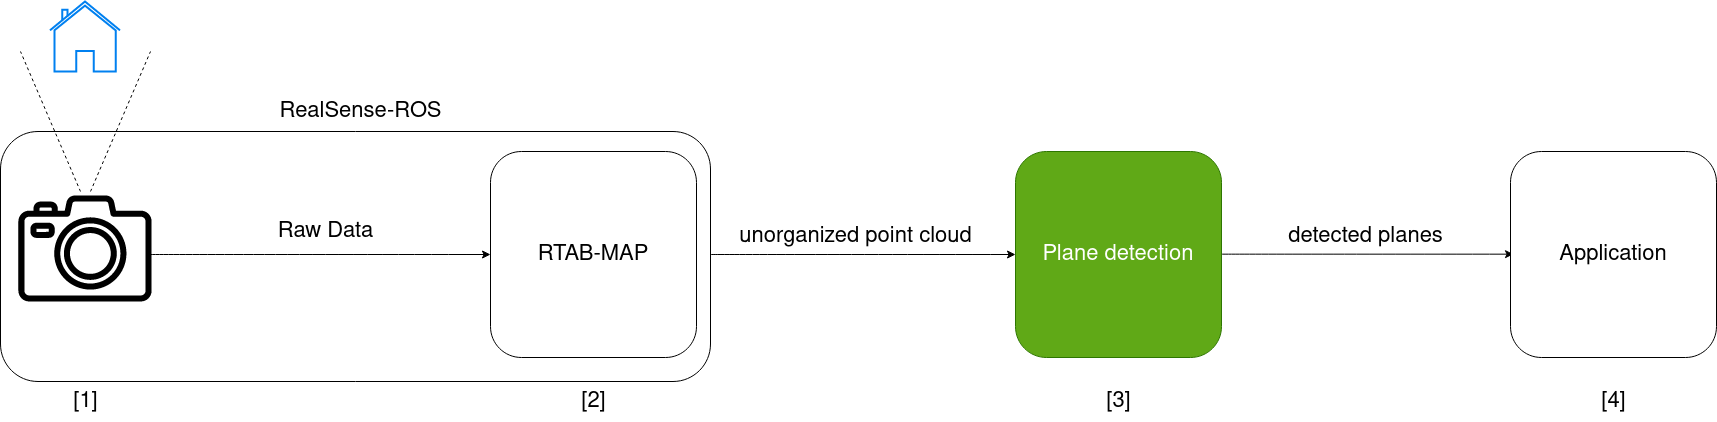
\includegraphics[width=15 cm]{images/concept_specific.png}
    \def\svgwidth{\textwidth}
    \input{images/conceptfig2.pdf_tex}
    \caption[AR/VR System]{A general view on an AR/VR system's architecture. The specialized sensor records data ([1]), which is passed to
        a SLAM algorithm ([2]). After map assembly, a point cloud is handed to a plane detection algorithm ([3]).
        The detected planes are given to a use-case-specific application ([4]).}
    \label{fig:concept}
\end{figure}

Many AR/VR Systems integrate plane detection into their software\footnote{\href{https://measurekit.com/}{https://measurekit.com/}}\footnote{\href{https://www.locometric.com/roomscan}{https://www.locometric.com/roomscan}}\footnote{\href{https://www.housecraftapp.com/}{https://www.housecraftapp.com/}}.
Figure~\ref{fig:concept} shows a generic block diagram of such a AR/VR system including plane detection.
The environment is continuously recorded by a specialized sensor, which is usually a camera, a depth sensor, or a combination thereof ([1]). A SLAM algorithm then integrates the new data into its already existing map ([2]). The map, in form of a point cloud, is subsequently passed to a plane detection algorithm ([3]). The algorithm performs the necessary steps to detect all planes inside the current map and passes the planes to the application ([4]).
The application then further processes those planes as required by the underlying use case.

To remove any noticeable delay in the application, the plane detection step has to run within a specific time limit. This temporal constraint is usually referred to as \textit{real-time}. \citeauthor{Davison_2003}~\cite{Davison_2003} observe that \textit{real-time} is usually bound to the sensor's frequency.
Motivated by this, we introduce a precise definition of \textit{real-time} in Section~\ref{sec:realtime}.

When creating such an AR/VR system, the choice of plane detection algorithm is naturally of great importance. The problem is that most published algorithms are inherently incomparable.
Often different datasets or metrics are used, which precludes a quantitative comparison.
Moreover, algorithms are often incomparable by internal functionality due to differences in inputs and the format of the detected planes. Plane detection algorithms are, in some cases, developed to run on specific hardware~\cite{gpuhough,Mols_Li_Hanebeck_2020}.
We can safely conclude that selecting a single 'best' algorithm, solely based on the results presented in their respective work, is impossible.

Motivated by Chapter~\ref{chap:Introduction}, we aim to determine the \textit{real-time} applicability in a realistic environment. To achieve this, we perform a uniform comparison of suitable plane detection algorithms. Therein, we especially pay attention to the accuracy and the calculation times.
This comparison will thereby yield the algorithm that produces the best results as well.
However, to perform this evaluation, we need the following:

\begin{enumerate}
    \item \label{enum:pda}Appropriate plane detection algorithms,
    \item \label{enum:ds} a realistic dataset, \textit{and}
    \item \label{enum:rt} a definition of \textit{real-time}.
\end{enumerate}
The following sections are dedicated to these requirements.

\section{Selection of Plane Detection Algorithms}\label{sec:pdaselection}
Since most algorithms differ in certain aspects, it is not possible to perform a comparison that includes every single one.
Furthermore, not all algorithms are created from the same motivation and focus on different things.
Evaluating an algorithm in a scenario it has not been designed for is likely to yield meaningless results.
It is, therefore, necessary to first define objective criteria upon which algorithms are judged to select suitable candidates for the remainder of this work.


\subsection{Criteria}
\label{subsec:criteria}
In the following paragraphs, we outline appropriate criteria for the objective assessment of plane detection algorithms.

\paragraph{Type of Input}\label{par:input}
The first criterion is the type of input expected by a plane detection algorithm.
Allowing vastly different inputs is likely to render the evaluation more complicated, if not impossible, because an equivalent transformation
between two input types is not always possible.

We detail the different types of input in Section~\ref{sec:dataformats}. To reiterate, the data representation of the recorded
environment falls into one of four categories:
\begin{itemize}
    \item unorganized or unstructured point cloud (UPC),
    \item organized or structured point cloud (OPC),
    \item Depth-Image (DI), \textit{and}
    \item RGB-Image (RGBI),
\end{itemize}
whereas OPC and UPC both describe point clouds in the cartesian coordinate system. The primary difference is that the 3D coordinates inside
an organized point cloud are saved in a 2D grid, while the unorganized point cloud resembles an unsorted 1D array. Moreover, the
Like OPC, depth images are a 2D grid of values. However, in contrast to the 3D coordinates of an OPC, the data points of depth images
are the distances to the sensor.

Depth images, like OPCs are arranged in a two-dimensional grid, while the included values are the distances to the sensor instead of 3D coordinates. The only difference between RGB and depth images is that the RGB image values are colored pixels.

\paragraph{Detected Plane Format} \label{subsec:planeformat}
It is essential to determine an appropriate representation of the detected planes.
If no uniform output type can be determined, consequently, no uniform metric for comparison can also be found.

In this work, we differentiate between the following:
\begin{itemize}
    \item 3D-inliers (3D-IN),
    \item 2D-inliers (2D-IN), \textit{and}
    \item the plane's normal vector and distance to origin ($n,d$),
\end{itemize}
whereas the 3D-inliers of a plane are a set of 3D points in the format of an UPC.
In contrast, 2D-inliers are two-dimensional representations of a plane.
This includes all methods to describe a plane in a two-dimensional manner, e.g., sets of indices, pixels or segmentation masks. These plane formats generally correspond to two-dimensional input formats like organized point clouds or (depth-) images.
Lastly, planes are often described mathematically over their normal vector $n$ and distance to the origin $d$.

\paragraph{Hardware Requirements}
\label{par:hardware}
Another important aspect to consider is the hardware required by an algorithm.
Most plane detection algorithms run on the CPU, some even implement some form of CPU parallelism, e.g., 3D-KHT uses OpenMP\footnote{\href{https://www.openmp.org/}{https://www.openmp.org/}}
to speed up the octree construction~\cite[Section~4]{LimbergerOliveira2015HT3D}.
However, some methods are implemented either completely or partially on the GPU.
For instance, \citeauthor{Hidalgo-Paniagua_Vega-Rodriguez_Pavón_Ferruz_2015}~\cite{Hidalgo-Paniagua_Vega-Rodriguez_Pavón_Ferruz_2015} compare different
implementations of the RANSAC algorithm, whereas three versions are processed entirely on the CPU, and the last one is offloaded
to the GPU via CUDA\footnote{\href{https://developer.nvidia.com/cuda-toolkit}{https://developer.nvidia.com/cuda-toolkit}}.

To summarize, we differentiate between algorithms that run solely on the CPU and algorithms that, additionally, employ the
machine's GPU.

\paragraph{Availability}
Lastly, to evenly compare a set of algorithms, all need to be implemented on the same machine to exclude the used hardware as a factor. Some authors provide a corresponding implementation to the paper in which they propose their novel plane detection technique. While other publications are limited to the paper, the level of detail regarding the implementation varies.


For further reference, we consider a plane detection algorithm to be \textit{available} if an implementation is generally possible, i.e.,  the authors provide their implementation or outline the algorithm in a way that enables self-implementation or a corresponding implementation is available online.

\subsection{Plane Detection Algorithms}
\label{subsec:pdaselect}
A list of state-of-the-art algorithms is compiled through comprehensive research of the current literature on plane detection (see Table~\ref{tab:algos}).
The table shows the input type and the output format of all algorithms, as well as the required hardware, and the availability.
Note that we consider all algorithms to be available. However, we are not aware of public implementations of OBRG and SCH-RG.
However, the respective publications outline their methods in high detail, thereby guiding a self-implementation.

The final outputs of PlaneNet, PlaneRecNet and PlaneRCNN are piecewise-planar depth maps of the input
image. Since modifying the architecture to return the segmentation masks and plane parameters would require minimal effort,
we adjusted the output types in the table accordingly. Similarly, RSPD returns a set of planes parameterized by
its normal vector $n$, distance to origin $d$, and two additional extents. Modifying the output to return inliers requires
minimal effort as well.
\begin{table}[H]
    \centering
    \caption[State-of-The-Art Plane Detection Algorithms]{A list of Plane Detection Algorithms compiled by reviewing the current literature. The algorithms are clustered by their type of input.
        The Section column provides the placement within this work. We refer to Subsection~\ref{subsec:criteria} for details regarding the specific namings of different plane formats. In the Hardware column, note that GPU implies the usage of the CPU.}
    \resizebox{\textwidth}{!}{%
        \begin{tabular}{cccccc}
            \toprule
            \textbf{Plane Detection Algorithm}                      & \textbf{Section}            & \textbf{Input Data} & \textbf{Plane Format} & \textbf{Hardware} & \textbf{Available} \\
            \midrule
            RSPD \cite{Araújo_Oliveira_2020}                        & \ref{subsec:bg-rspd}        & UPC                 & 3D-IN, $(n,d)$        & CPU               & Y                  \\
            OPS \cite{Sun_Mordohai_2019}                            & \ref{subsec:bg-ops}         & UPC                 & 3D-IN                 & CPU               & Y                  \\
            3DKHT \cite{LimbergerOliveira2015HT3D}                  & \ref{subsec:bg-3dkht}       & UPC                 & 3D-IN                 & CPU               & Y                  \\
            OBRG \cite{Vo_Truong-Hong_Laefer_Bertolotto_2015}       & \ref{subsec:bg-obrg}        & UPC                 & 3D-IN                 & CPU               & Y                  \\
            PEAC \cite{Feng_Taguchi_Kamat_2014}                     & \ref{subsec:bg-peac}        & OPC                 & 2D-IN                 & CPU               & Y                  \\
            CAPE \cite{Proença_Gao_2018}                            & \ref{subsec:bg-cape}        & OPC                 & $(n, d)$              & CPU               & Y                  \\
            SCH-RG \cite{Mols_Li_Hanebeck_2020}                     & \ref{subsec:bg-schrg}       & OPC                 & 2D-IN                 & GPU               & Y                  \\
            D-KHT  \cite{Vera_Lucio_Fernandes_Velho_2018}           & \ref{subsec:bg-dkht}        & DI                  & 2D-IN                 & CPU               & Y                  \\
            DDFF \cite{Roychoudhury_Missura_Bennewitz_2021_new}     & \ref{subsec:bg-ddff}        & DI                  & 2D-IN                 & CPU               & Y                  \\
            PlaneNet \cite{Liu_Yang_Ceylan_Yumer_Furukawa_2018}     & \ref{subsec:bg-planenet}    & RGBI                & 2D-IN, $(n, d)$       & GPU               & Y                  \\
            PlaneRecNet \cite{Xie_Shu_Rambach_Pagani_Stricker_2022} & \ref{subsec:bg-planerecnet} & RGBI                & 2D-IN, $(n)$          & GPU               & Y                  \\
            PlaneRCNN \cite{Liu_Kim_Gu_Furukawa_Kautz_2019}         & \ref{subsec:bg-planercnn}   & RGBI                & 2D-IN, $(n, d)$       & GPU               & Y                  \\
            \bottomrule
        \end{tabular}
    }
    \label{tab:algos}
\end{table}

As mentioned above, we consider all presented algorithms available even if SCH-RG and OBRG do not seem to have an official implementation.
Therefore, while necessary, the criterion of availability does not constrain the selection of algorithms in this case.

Integrating an external GPU into the system poses an additional cost factor. Moreover, the additional weight could have negative effects on the user experience, as AR/VR devices are usually handheld or head-worn.
We exclude algorithms that require an external GPU, namely SCH-RG, PlaneNet, PlaneRecNet, and PlaneRCNN.

Addressing the criterion of input type, we are only interested in performing plane detection in complete environments.
Each update published by RTAB-MAP is the union of new data and the current state of the recorded map. RTAB-MAP publishes this update in form of an unorganized point cloud (see Figure~\ref{fig:rtabmap}).
To perform plane detection with an algorithm that expects an OPC as input, the UPC has to be transformed into an OPC.
This transformation is not-trivial and involves the projection of 3D coordinates onto a sphere based on a set of sensor parameters.
An exemplary implementation thereof is included in the lidar toolbox of MATLAB\footnote{\href{https://de.mathworks.com/help/lidar/ug/unorgaized-to-organized-pointcloud-conversion.html}{https://de.mathworks.com/help/lidar/ug/unorgaized-to-organized-pointcloud-conversion.html}}.
However, this transformation neglects the global structure of the environment, as it returns a two-dimensional representation of the environment.
Therefore, we focus on unorganized point clouds in this work and exclude PEAC, CAPE, SCH-RG, D-KHT, DDFF, PlaneNet, PlaneRecNet and PlaneRCNN from our evaluation.

The detected planes need to be in the same format because, even for the same plane, different representations could very well lead to different results.
Assume a plane in cartesian form ($n,d$) and a plane represented by its (3D/2D) inliers. The calculated metrics may differ significantly because the plane in cartesian form is infinitely dense.
Conversely, the plane described by its inliers allows for holes and non-rectangular shapes, e.g., doorways or a round table, respectively.
Being able to represent planes of arbitrary shape is important for many applications. Moreover, only the 3D inliers (3D-IN) conform to
the determined input type of UPC (see Section~\ref{subsec:output}).
We thereby determine 3D-IN as the preferred plane format and exclude all methods which do not comply, namely CAPE, PlaneNet, PlaneRecNet, and PlaneRCNN.
Note that, hereafter, we refer to 3D-IN solely as inliers.


Finally, we end up with, and thus include, the following plane detection algorithms in our evaluation:

\begin{multicols}{4}
    \begin{itemize}
        \item[\vspace{\fill}]
        \item[\vspace{\fill}]
        \item \textbf{RSPD}
        \item \textbf{OPS}
        \item \textbf{3D-KHT}
        \item \textbf{OBRG}
        \item[\vspace{\fill}]
        \item[\vspace{\fill}]
    \end{itemize}

\end{multicols}

\paragraph{Temporal Subdivision of Phases}
\label{par:prepostalgos}
To enable a precise evaluation, we subdivide these algorithms into a pre-processing phase, a plane detection phase, and a post-processing phase, whereas we use the terms "phase" and "step" interchangeably in this work. In the following, we outline the pre-processing and post-processing steps taken by the selected algorithms. To avoid redundancy,
we refer the reader to the Subsections~\ref{subsec:bg-rspd}-\ref{subsec:bg-obrg} for more details regarding the plane detection steps of each algorithm.

The pre-and post-processing steps are summarized in Table~\ref{tab:pre-post}.
RSPD, 3D-KHT, and OBRG construct an octree (OC) during their pre-processing phase.
Additionally, RSPD and OBRG perform an initial estimation of normals (NE).
OPS estimates the normal vectors for a randomly chosen sample set of points of pre-determined size.

During post-processing, OPS merges smaller planes if they pass a coplanarity test and then re-estimates the normals of the
resulting plane.
In the post-processing step, OBRG refines the borders of detected planes by inserting previously unallocated regions. RSPD and 3D-KHT do not perform post-processing.

\begin{table}[H]
    \centering
    % \parbox{0.7\textwidth}{\caption[Pre-processing \& Post-processing Phases of Selected Algorithms]{The Pre-processing and post-processing steps of the plane detection algorithms. "/" denotes the absence of
    %         a pre-/post-processing step.}
    % }
    \caption[Pre-processing \& Post-processing Phases of Selected Algorithms]{The Pre-processing and post-processing steps of the plane detection algorithms. "/" denotes the absence of a pre-/post-processing step.}
    \label{tab:pre-post}
    % \resizebox{0.7\textwidth}{!}{%
    \begin{tabular}{ccccc}
        \toprule
        \textbf{Phase}  & \textbf{RSPD} & \textbf{OPS} & \textbf{3D-KHT} & \textbf{OBRG} \\
        \midrule
        Pre-processing  & NE            & NE           & OC              & OC + NE       \\
        Post-processing & /             & Merge        & /               & Refinement    \\
        \bottomrule
    \end{tabular}
    % }
\end{table}




\section{Selection of Datasets}
\label{sec:datasets}
After having obtained a set of suitable algorithms and, according to requirements introduced at the beginning of this chapter (see Section~\ref{enum:ds}), the selection of realistic dataset is necessary.
Just like a substantial amount of algorithms are incomparable for different reasons, datasets differ in certain aspects as well.
Therefore, this section deals with the selection of an appropriate dataset.

\subsection{Criteria}
We introduce a set of criteria upon which currently popular datasets are compared. These criteria are widely influenced by the criteria used for the previous selection of algorithms (see Subsection~\ref{subsec:criteria}).

\paragraph{Scene Format}
\label{par:sceneformat}
The Format of a scene in a given dataset corresponds directly to the input of algorithms.
To avoid redundancy, we refer the reader to Subsection~\ref{subsec:input} and Paragraph~\ref{par:input} for more information.
Thereby, the scene format can be divided into the same four classes:
\begin{itemize}
    \item unorganized or unstructured point cloud (UPC)
    \item organized or structured point cloud (OPC)
    \item Depth-Image (DI)
    \item RGB-Image (RGBI)
\end{itemize}

\paragraph{Realism}
We differentiate between synthetic and real/realistic datasets.
Real datasets represent real environments, as they are often recorded manually.
In contrast, synthetic datasets often include a collection of geometric bodies and are usually created digitally.
Two representatives for both types are shown in Figure~\ref{fig:ds_realism}.

\paragraph{Recorded Environment}
Since realistic datasets are created through manual recording, it is useful to
differentiate between indoor and outdoor environments.
Note that we consider this criterion only to apply for real datasets as synthetic
datasets are not recorded manually.

\begin{figure}[H]
    \centering
    \hspace{\fill}
    \begin{subfigure}{0.3\textwidth}
        \centering
        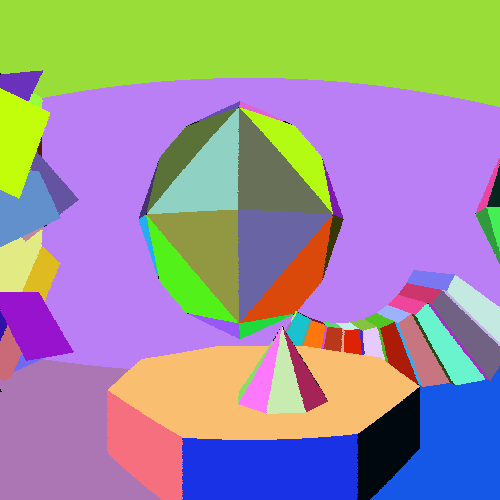
\includegraphics[width=\textwidth]{images/synthetic_ds.png}
        \caption[Synthetic Dataset Example]{}
        \label{fig:synth}
    \end{subfigure}
    \hspace{\fill}
    \begin{subfigure}{0.45\textwidth}
        \centering
        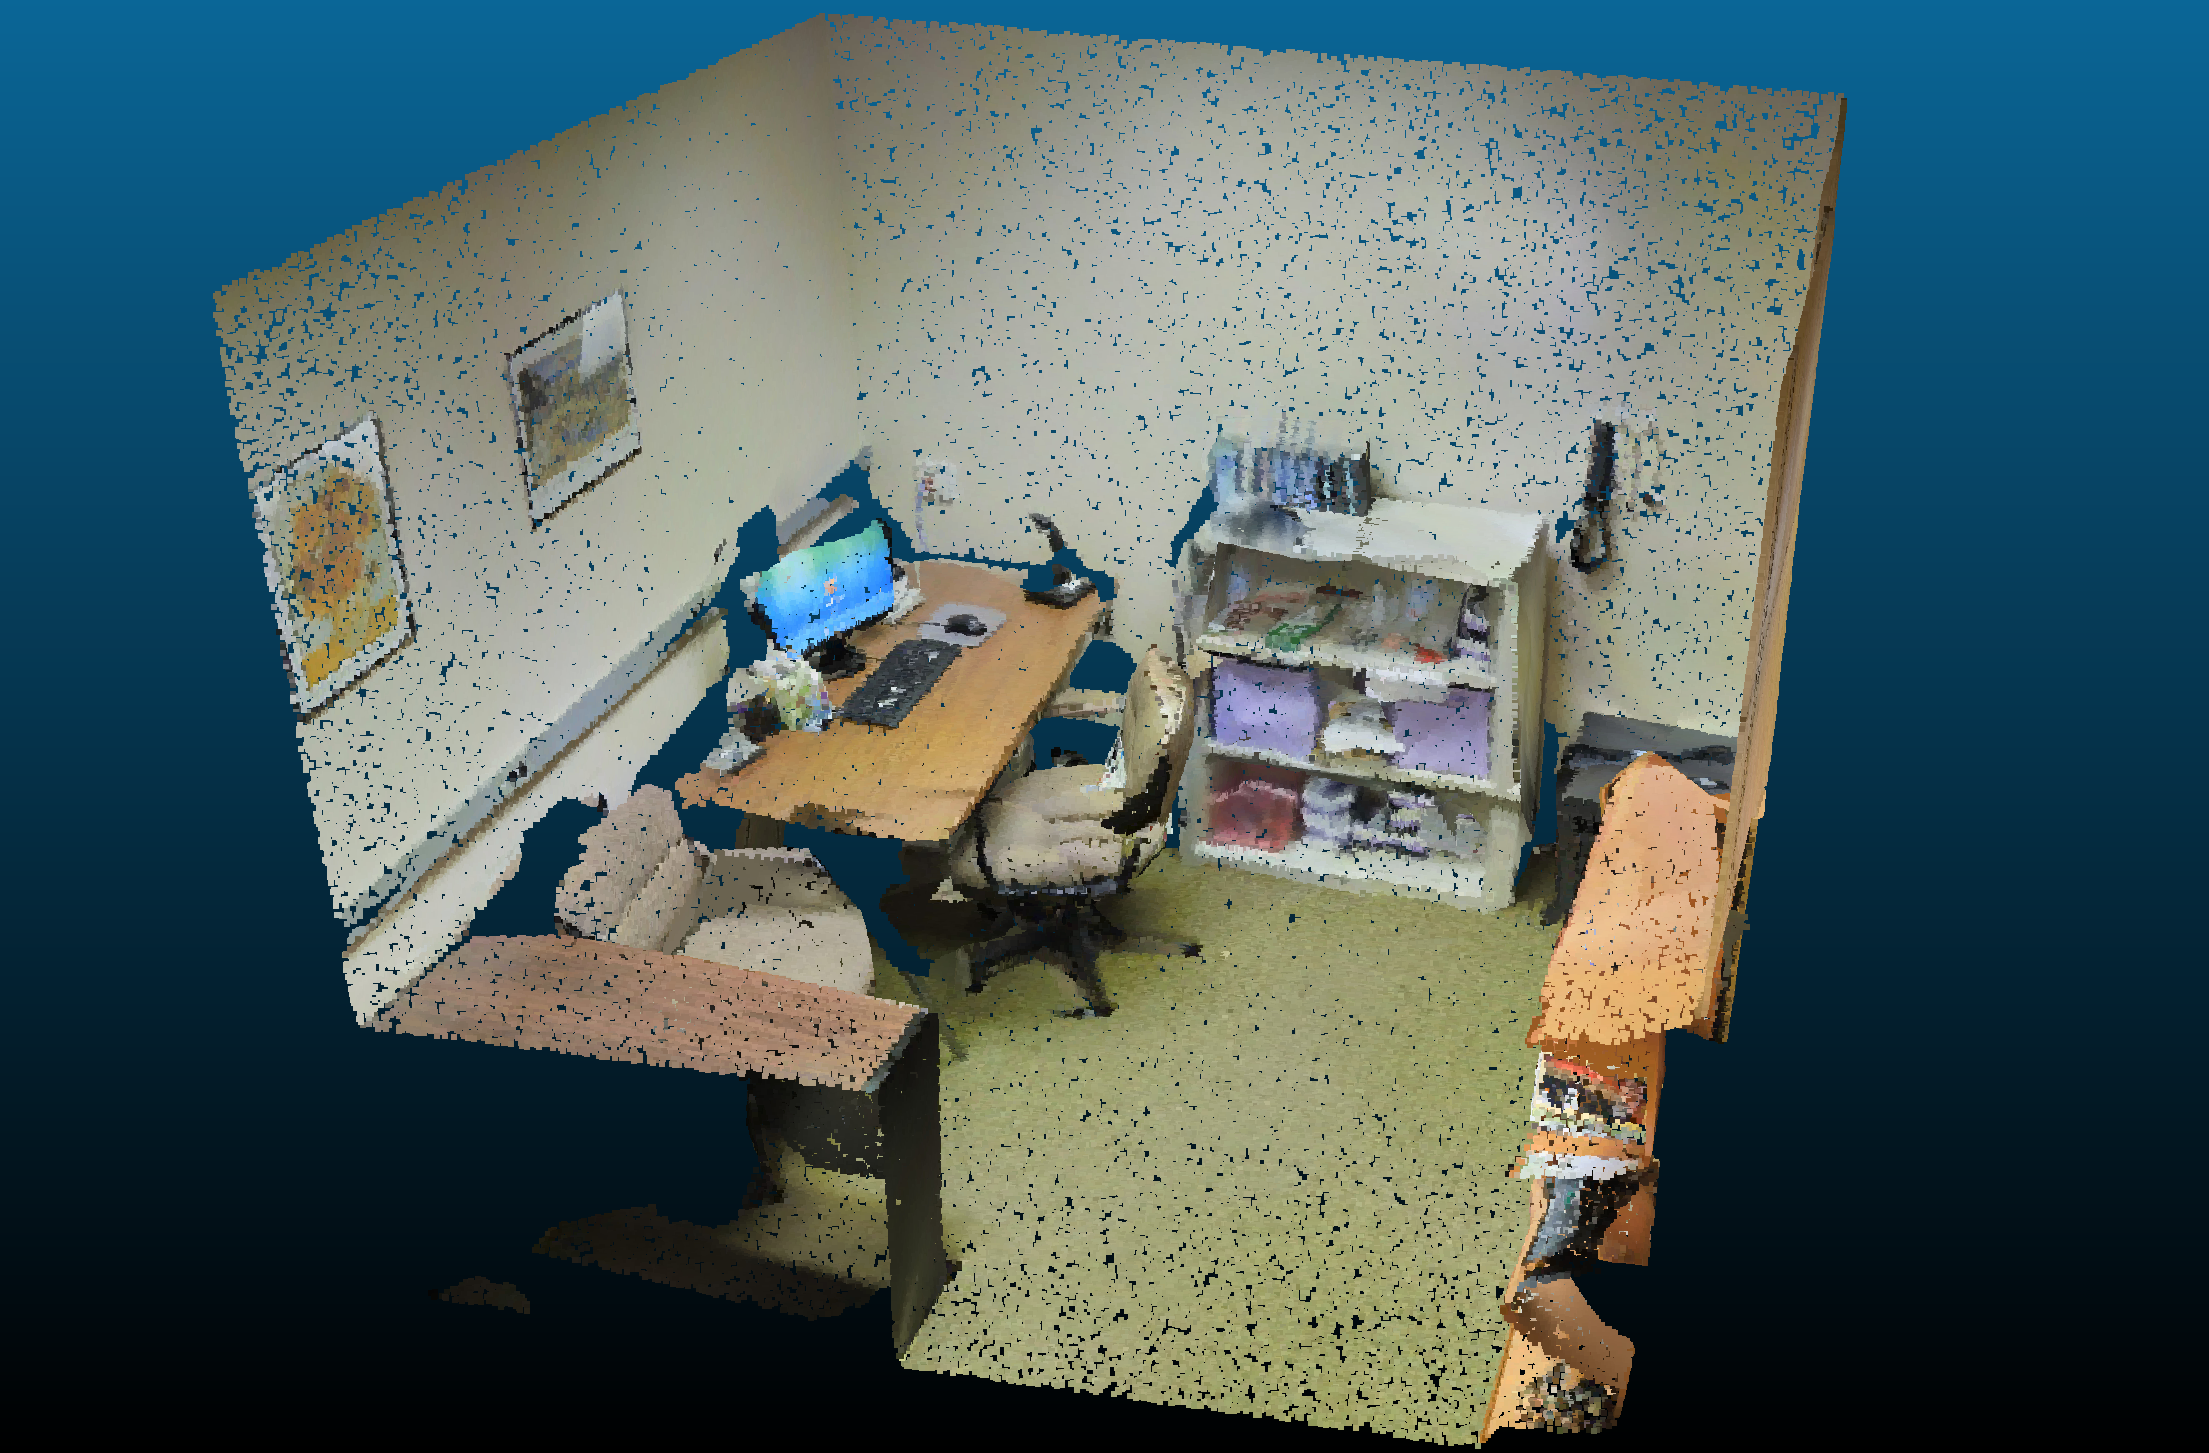
\includegraphics[width=\textwidth]{images/real_ds.png}
        \caption[Realistic Dataset Example]{}
        \label{fig:real}
    \end{subfigure}
    \hspace{\fill}
    \caption[Synthetic and Realistic Dataset Comparison]{A synthetic dataset (a) and a real office scene (b).
        The former is from the \textit{SegComp}~\cite{article} dataset, and the latter is from the 2D-3D-S~\cite{2017arXiv170201105A} dataset.
        Note that we cropped the office point cloud for visualization purposes.}
    \label{fig:ds_realism}
\end{figure}



\paragraph{Ground Truth}
Lastly, not all datasets are created out of the same motivation. Therefore, the method of evaluation differs widely over the range of available datasets.
In general, the ground truth (GT) of currently popular datasets can fall into one of the following categories (compare Table~\ref{tab:datasets}):

\begin{itemize}
    \item Planes,
    \item classes, \textit{or}
    \item trajectory.
\end{itemize}
In some datasets, the ground truth represents a set of detectable planes.
The specific
Therein, the format of the planes depends on the plane format of the algorithm (see Paragraph~\ref{subsec:planeformat}).

Often, datasets from the field of semantic segmenation or object detection are used for the evaluation of plane detection algorithms.
Therein, objects in a scene are assigned specific object classes, e.g., "Wall", "Ceiling", "Table", or "Cup".
The ground truth provides a labeling of these objects. This labeling can take the form of annotated 3D bounding boxes or sets of pixels in the input image.

Lastly, some datasets provide a GT that focuses on the trajectory of the recording sensor. This trajectory is usually taken from integrated sensors like \textit{Inertial Measurement Units} (IMUs).

Naturally, this classification can only apply to datasets that include a ground truth.

\subsection{Datasets}
Table~\ref{tab:datasets} summarizes currently prevalent datasets in the scientific literature regarding plane detection.
Most of the datasets therein are used in the corresponding papers of the plane detection algorithms presented in Table~\ref{tab:algos}.
However, this does not influence the selection process. Note that SYNPEB and SegComp are synthetic datasets and, therefore, are neither indoor nor outdoor.
Furthermore, we are not aware of a ground truth for the ARCO dataset.

\begin{table}[H]
    \centering
    \caption[State-of-The-Art Datasets]{Plane detection Datasets. The GT column specifies what the ground truth of each dataset represents.
        The datasets are clustered by their type of format.
        The second column provides the placement within this work.
        Note that we include our $FIN$ dataset in this table for completeness reasons.
    }

    \resizebox{\textwidth}{!}{%
        \begin{tabular}{cccccc}
            \toprule
            \textbf{Dataset}                                                                                                                                                             & \textbf{Section}         & \textbf{Scene Format} & \textbf{Real} & \textbf{Indoor} & \textbf{GT} \\
            \midrule
            2D-3D-S      \cite{2017arXiv170201105A}                                                                                                                                      & \ref{subsec:bg-stanford} & UPC                   & Y             & Y               & classes     \\
            Leica\tablefootnote{\href{https://shop.leica-geosystems.com/de/leica-blk/blk360/dataset-downloads}{https://shop.leica-geosystems.com/de/leica-blk/blk360/dataset-downloads}} & \ref{subsec:bg-Leica}    & UPC                   & Y             & N               & planes      \\
            Kinect     \cite{Oehler_Stueckler_Welle_Schulz_Behnke_2011}                                                                                                                  & \ref{subsec:bg-Kinect}   & OPC                   & Y             & Y               & planes      \\
            SYNPEB      \cite{schaefer19icra}                                                                                                                                            & \ref{subsec:bg-SYNPEB}   & OPC                   & N             & /               & planes      \\
            ARCO       \cite{Hidalgo-Paniagua_Vega-Rodriguez_Pavón_Ferruz_2015}                                                                                                          & \ref{subsec:bg-ARCO}     & OPC                   & Y             & Y               & /           \\
            SegComp     \cite{article}                                                                                                                                                   & \ref{subsec:bg-segcomp}  & DI                    & N             & /               & planes      \\
            NYU V2      \cite{10.1007/978-3-642-33715-4_54}                                                                                                                              & \ref{subsec:bg-NYU}      & DI                    & Y             & Y               & classes     \\
            ICL-NUIM    \cite{handa:etal:ICRA2014}                                                                                                                                       & \ref{subsec:bg-ICL}      & DI                    & Y             & Y               & trajectory  \\
            SUNRGB-D         \cite{7298655}                                                                                                                                              & \ref{subsec:bg-SUN}      & DI                    & Y             & Y               & classes     \\
            TUM         \cite{sturm12iros}                                                                                                                                               & \ref{subsec:bg-TUM}      & DI                    & Y             & Y               & trajectory  \\
            \midrule
            FIN (ours)                                                                                                                                                                   & \ref{sec:finimpl}        & UPC                   & Y             & Y               & planes      \\
            \bottomrule
        \end{tabular}
    }
    \label{tab:datasets}
\end{table}


In Subsection~\ref{subsec:pdaselect}, we determine unorganized point clouds as the type of input.
Furthermore, since we give special focus to the real-world applicability of plane detection algorithms, we must evaluate them on realistic datasets, thereby excluding all datasets except 2D-3D-S and Leica.
Additionally, we are especially interested in realistic $indoor$ environments, as motivated by Chapter~\ref{chap:Introduction}.
Therefore, Leica ceases to be an option and we subsequently choose 2D-3D-S as the dataset for the evaluation.

Nevertheless, we cannot use the ground truth included in 2D-3D-S because it represents the segmented scene at the level of objects~\cite[Section~4.1]{2017arXiv170201105A} instead of focusing on planes within the scene.
As a consequence thereof, we create a suitable ground truth of the 2D-3D-S dataset through manual segmentation.
We provide details of this time-expensive process in Section~\ref{sec:gtseg}.



Since the unorganized point clouds do not grow incrementally over time, 2D-3D-S does not inherit any temporal component.
Moreover, \citeauthor{2017arXiv170201105A}~\cite{2017arXiv170201105A} recorded the dataset with a static 360° camera. Therefore, the dataset is not entirely realistic, though being recorded in a real environment.


To our knowledge, no dataset meets the above criteria, is genuinely realistic, and includes a plane-focused ground truth.
Therefore, we record an incrementally growing dataset in the Faculty of Computer Science at Otto-von-Guericke University Magdeburg, namely  the FIN dataset.

To perform a comparison between the FIN and 2D-3D-S, we record a scene for each of the following scene types (see Figure~\ref{fig:fin}):
{\setlength\multicolsep{0pt}%
\begin{multicols}{2}
    \begin{itemize}%[noitemsep,topsep=0pt]
        \item auditorium
        \item hallway
        \item conference room
        \item office
    \end{itemize}
\end{multicols}
}
We focus on these four scene types because they are the most common in a realistic indoor environment.
Lastly, since this is a novel dataset, we need to create a ground truth. The details thereof are explained in Section~\ref{sec:finimpl}.

\begin{figure}[H]
    \centering
    \begin{subfigure}{0.4\textwidth}
        \centering
        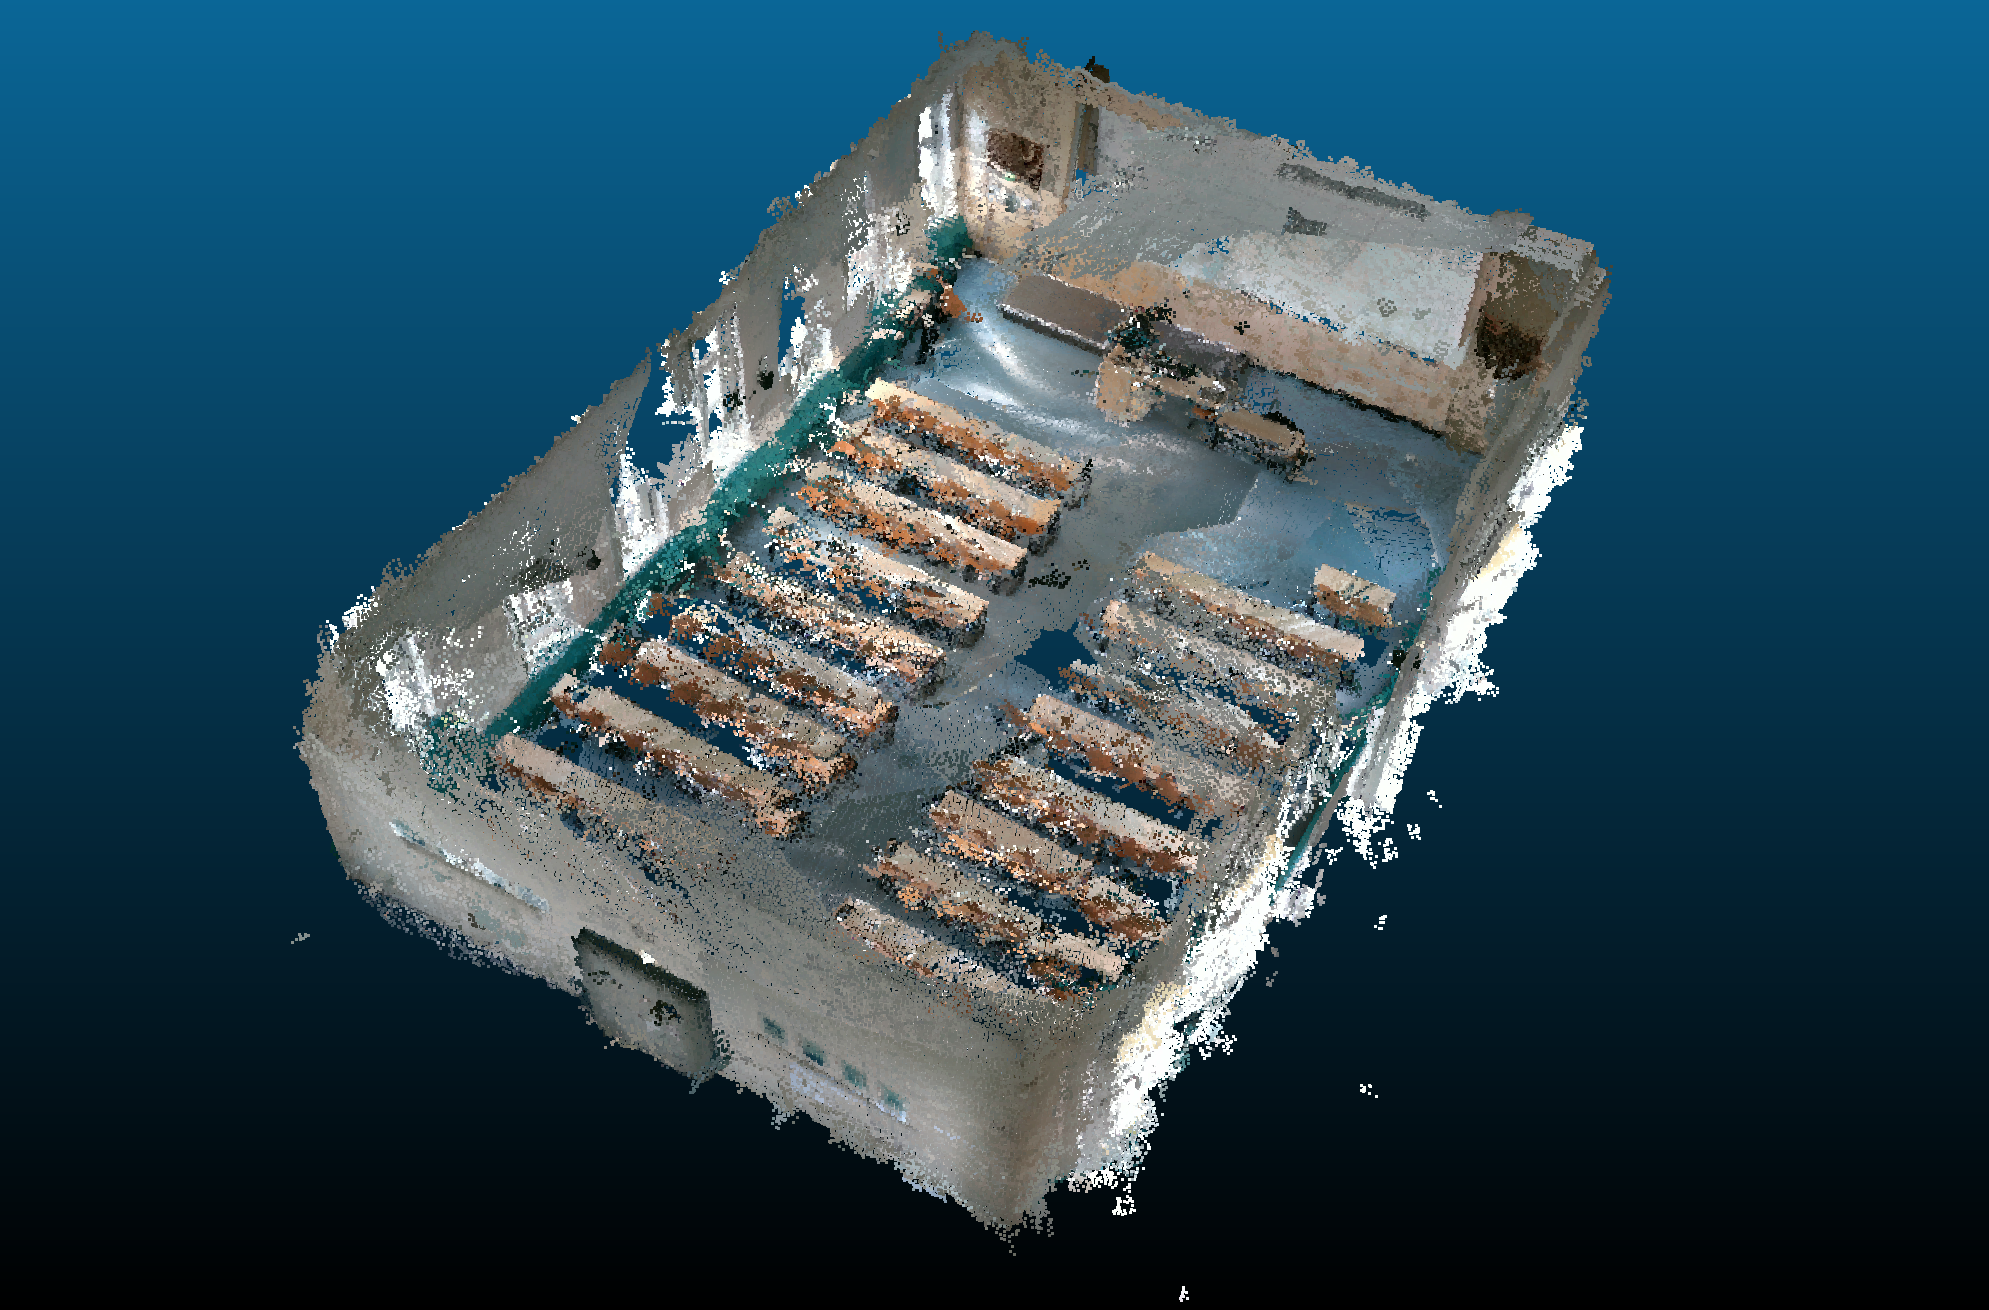
\includegraphics[width=.8\linewidth]{images/307.png}
        \caption[Auditorium Scene]{}
        \label{fig:fin307}
    \end{subfigure}
    \begin{subfigure}{0.4\textwidth}
        \centering
        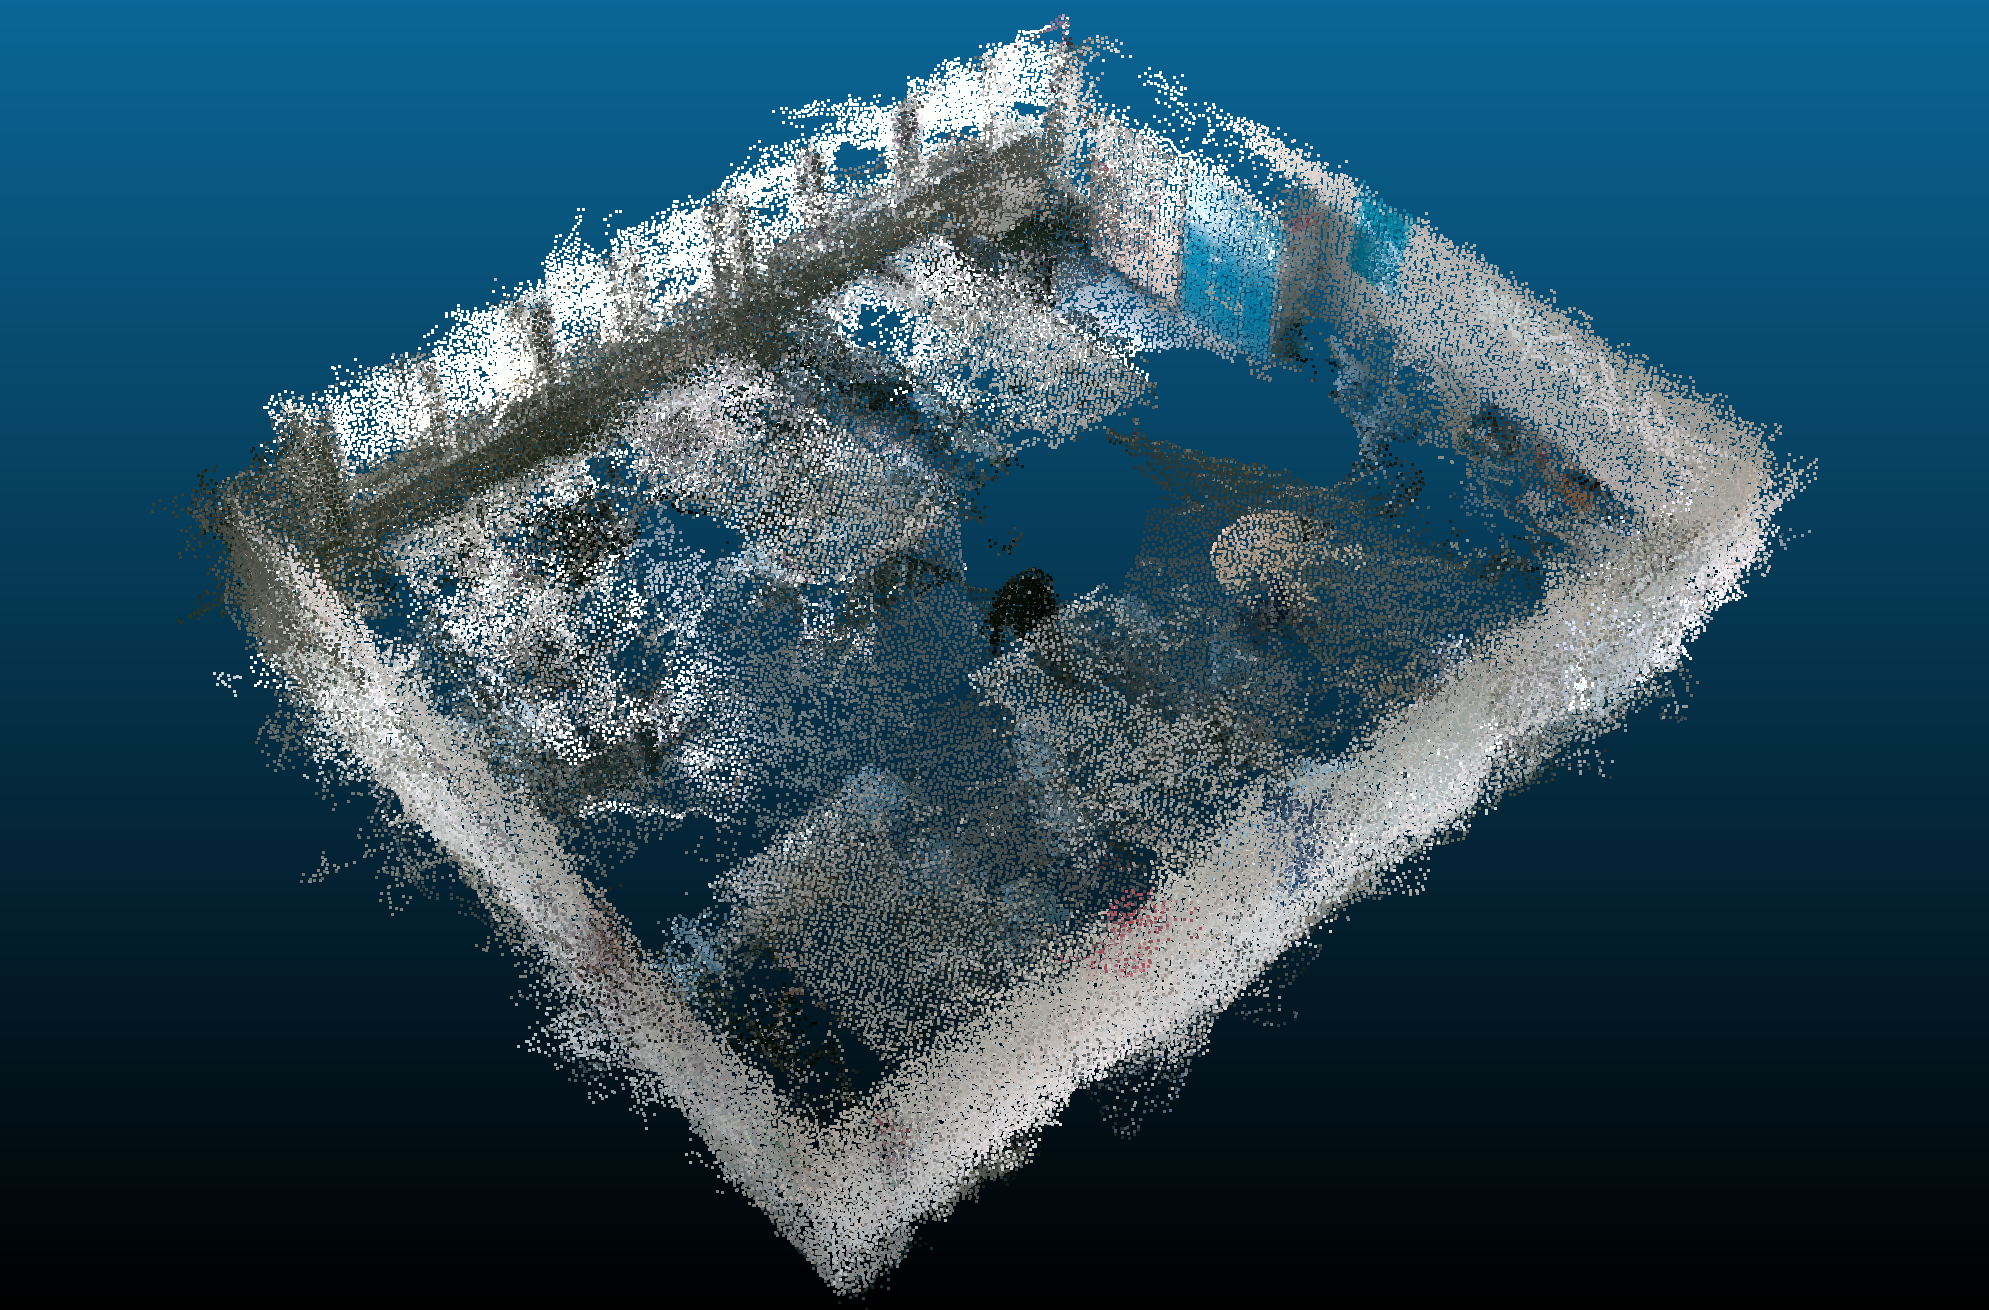
\includegraphics[width=.8\linewidth]{images/333.png}
        \caption[Conference Room Scene]{}
        \label{fig:fin333}
    \end{subfigure}
    \begin{subfigure}{0.4\textwidth}
        \centering
        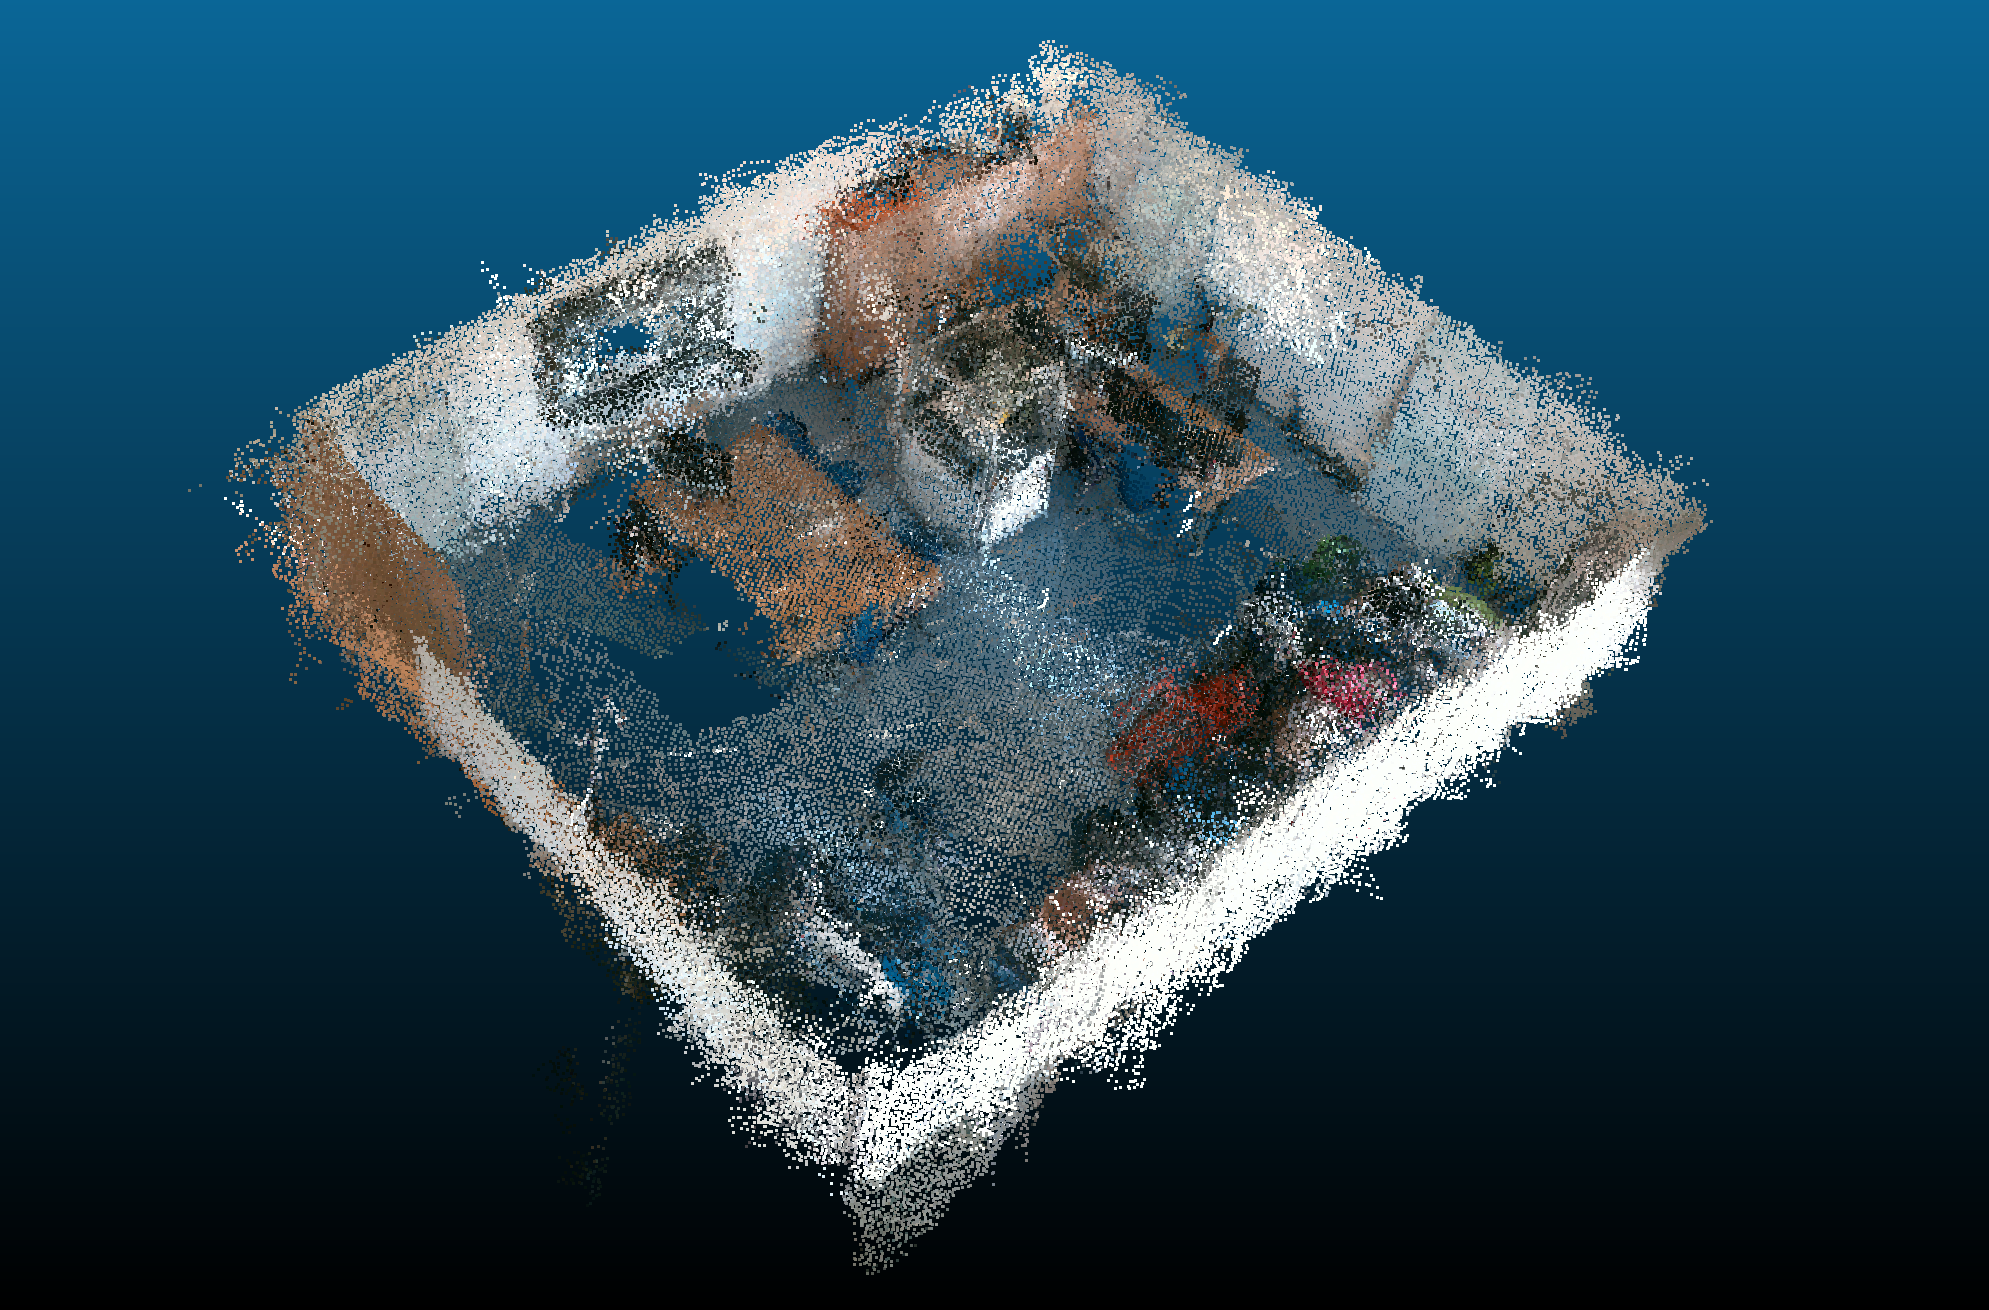
\includegraphics[width=0.8\linewidth]{images/425.png}
        \caption[Office Scene]{}
        \label{fig:fin425}
    \end{subfigure}
    \begin{subfigure}{0.4\textwidth}
        \centering
        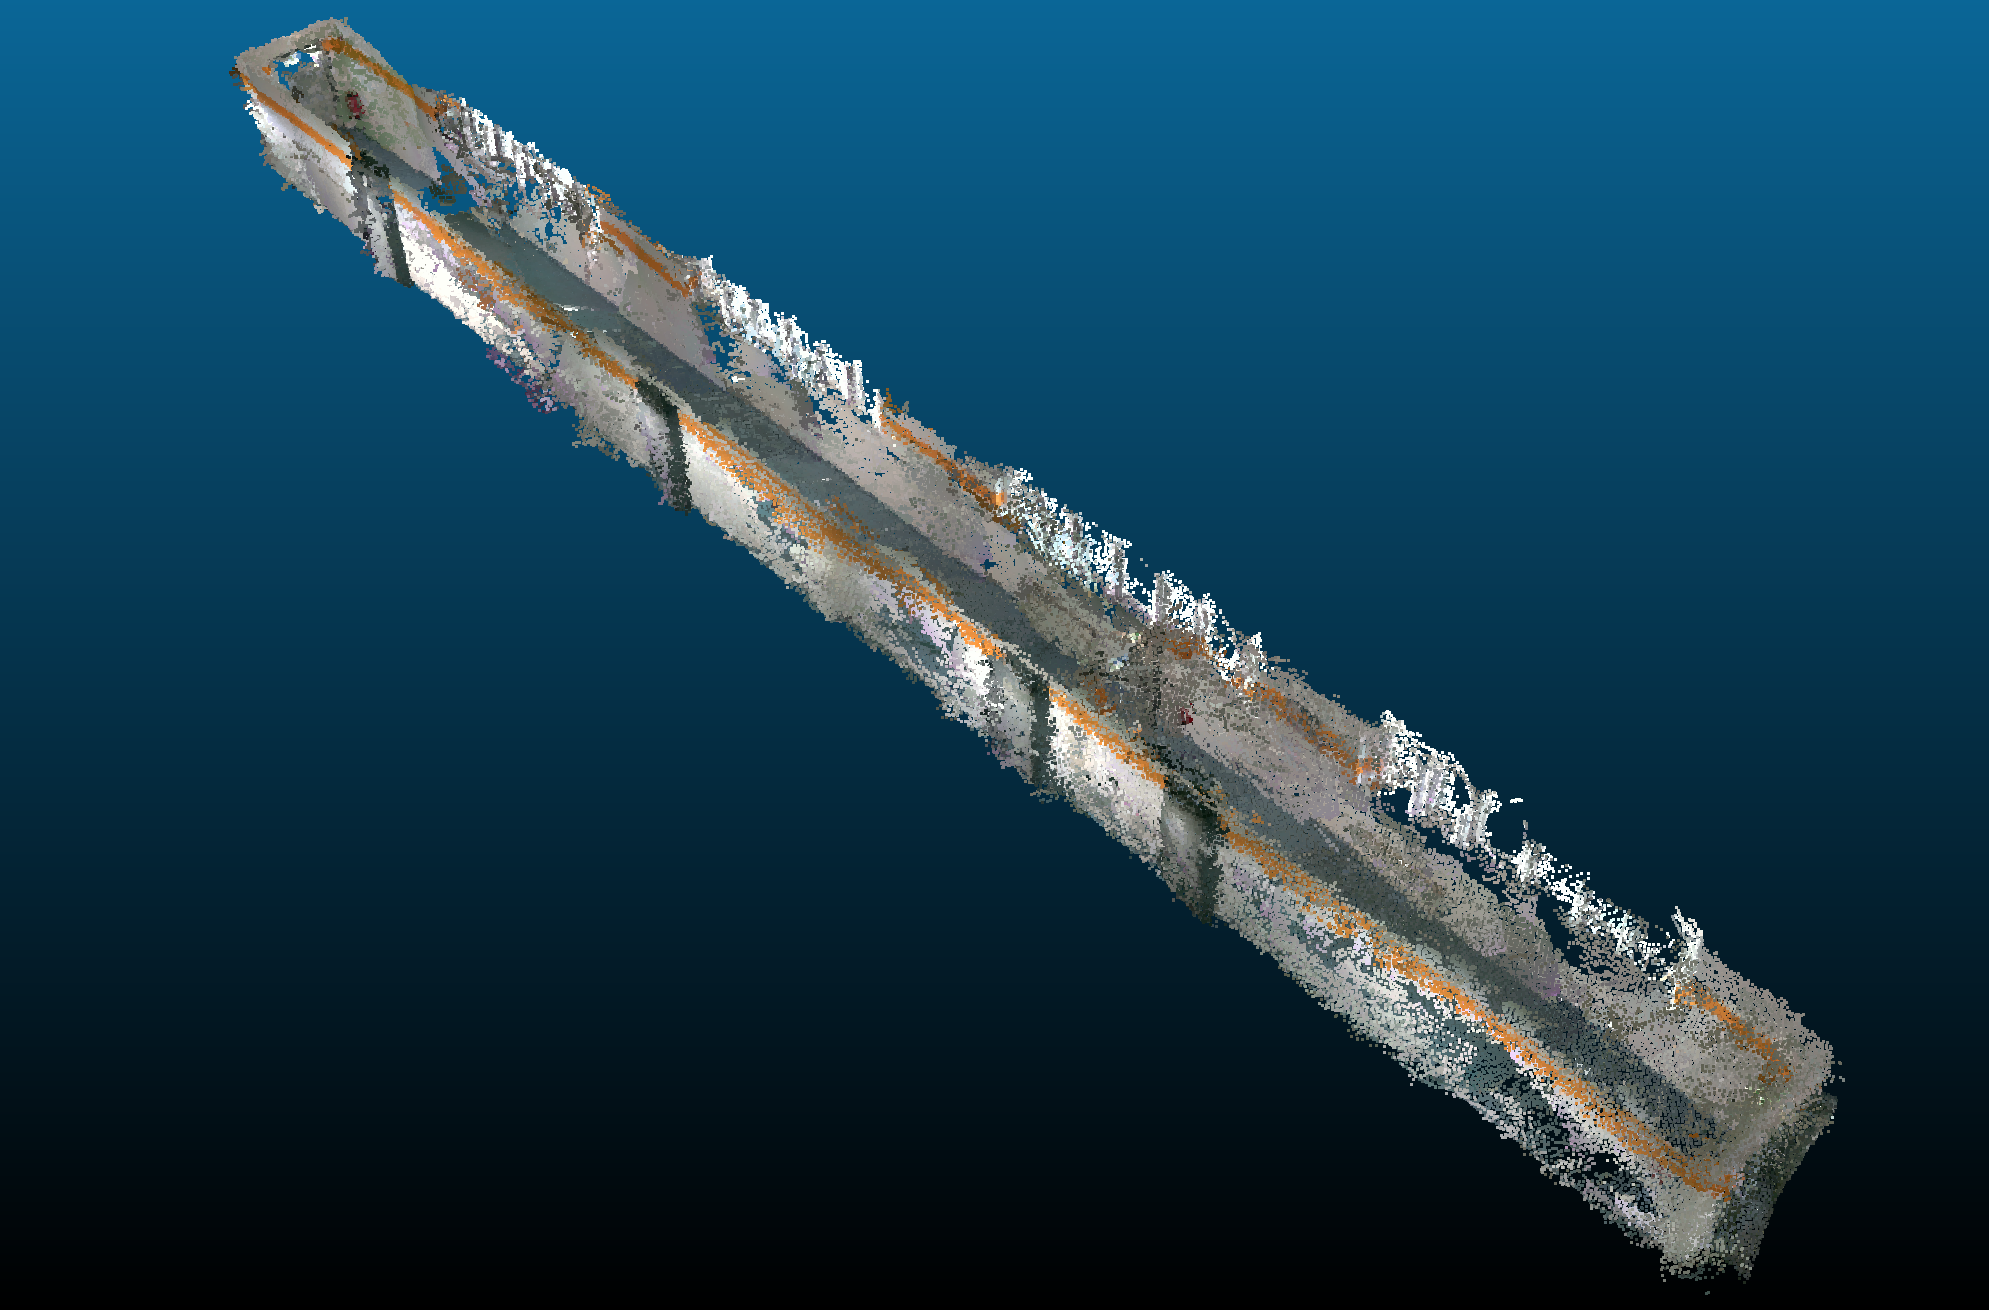
\includegraphics[width=0.8\linewidth]{images/hallway.png}
        \caption[Hallway Scene]{}
        \label{fig:finhw}
    \end{subfigure}
    \caption[FIN Dataset]{The recorded point clouds for each scene type: (a) $auditorium$, (b) \textit{conference room}, (c) \textit{office} and (d) $hallway$.
        The ceilings have been manually removed for visualization purposes but remain in the dataset for the experiments.
        Full-size figures can be found in Appendix~\ref{app:fin-scenes}}
    \label{fig:fin}
\end{figure}


\section{Definition Real-Time}\label{sec:realtime}
Finally, as mentioned in the beginning of this Chapter, we must define the meaning of \textit{real-time} to determine the \textit{real-time} applicability of a plane detection algorithm.

In Subsection~\ref{subsec:pdaselect}, we introduce the differentiation between pre-processing and post-processing steps.
It is possible that one phase of an algorithm accounts for the majority of the total calculation time and that the algorithm
would be considered \textit{real-time} applicable, if that phase were to be excluded.
Because some steps can be covered by previous steps in the AR/VR system (see Figure~\ref{fig:concept}), i.e., by the sensor or the SLAM algorithm,
we give two definitions of \textit{real-time}.

In general, and without taking the algorithms internal structure into consideration, we have to consider possible
hardware limitations, data flow, and how often it is needed to perform calculations, e.g., how quickly the SLAM algorithm
updates its internal map (Figure~\ref{fig:concept}, [2]) or how frequently new planes are needed (Figure~\ref{fig:concept}, [4]).
The recorded raw data is not directly sent to the plane detection algorithm but instead given to RTAB-MAP, which then performs
calculations to update and publish the map.
Therefore, the upper limit is the frequency of how often RTAB-MAP publishes those updates, which by default is once per second.

\paragraph{Total Real-Time $\mathbf{RT_{tot}}$}
According to this upper limit of RTAB-MAP, we consider an algorithm to have \textit{Total Real-Time} applicability, if it achieves an average frame
rate of minimum 1, i.e., the total processing time of an algorithm lies under one second. In the remainder of this work, we
use \textit{Total Real-Time} and $RT_{tot}$ interchangeably.

\paragraph{Real-Time Plane Calculation $\mathbf{RT_{calc}}$}
Being a subset of \textit{total Real-Time} applicability, \textit{Real-Time Plane Calculation} determines the \textit{real-time} applicability if the processing time of an algorithm
\textit{excluding} pre-processing lies under the aforementioned upper bound of $1s$. Like $RT_{tot}$, we use
\textit{Real-Time Plane Calculation} and $RT_{calc}$ interchangeably.

\section{Summary}
Many Augmented Reality applications have constraints in the form of a temporal component. Augmented or Virtual Reality applications that include plane detection are no exception. Thereby, these constraints apply to the plane detection algorithms as well. In addition to time constraints, good quality is often tightly coupled to expensive or closed technology.
In this work, we aim to evaluate the quality of \textit{real-time} plane detection algorithms under the use of more affordable hardware, namely two Intel RealSense sensors. Therein, we are especially interested in the aspect of \textit{real-time} applicability in a realistic environment.

At the beginning of this chapter, we state that three aspects are required for this evaluation: A set of plane detection algorithms, useful datasets, and a definition
of \textit{real-time}.
The selection of the best plane detection algorithm, however, is non-trivial. After defining meaningful criteria for objective judgement, we
select appropriate plane detection algorithms. Moreover, we select realistic datasets, one of which is a novel creation, and present two definitions of \textit{real-time} namely $RT_{tot}$ and $RT_{calc}$.
\end{document}